%----------------------------------------------------------%
% Beamer template for presentations within PPGCC PUCRS     %
% by Anderson Domingues (anderson.domingues@acad.pucrs.br) %
%                                                          %
% made over "Template Beamer para Apresentações da UFRN"   %
% by alcemygvseverino@gmail.com (ver. 1.1, 14/05/2016)     %
%----------------------------------------------------------%

\documentclass[aspectratio=169,handout,t,table]{beamer}

%\usepackage[table]{xcolor}
\usepackage[english]{babel}              % document language
\usepackage[utf8]{inputenc}              % utf-8 support
% \usepackage{multicol}

%\usepackage[alf]{abntex2cite}            % ABNT citation style

\usepackage[square, sort, comma, numbers]{natbib}
\usepackage{graphicx}
\usepackage{float}
\usepackage{geometry}
\usepackage{tikz}
\usepackage{amsmath}
\usepackage{amssymb}

\usepackage{multirow}

% \usepackage{url}
\usepackage{pgfpages}                   % allows including pdf

\usepackage{enumerate}
\usepackage{color}
\usepackage{ifthen}
\usepackage{capt-of}                    % support for caption 

\usepackage{soul}
\usepackage{booktabs}

\usepackage{pgfplots}
\usepackage{pgfplotstable}
\usepackage{svg}


% Background
% \setbeamertemplate{background}{
%     \includegraphics[width=\paperwidth,keepaspectratio]{template/sbcci24bg.png}
% }

% TikZ solution
\newcommand*\circnum[1]{\tikz[baseline=(char.base)]{
            \node[shape=circle,draw,inner sep=1.2pt] (char) {#1};}} 

\usetikzlibrary{arrows,shapes,fit,positioning,shadows,trees,calc,pgfplots.groupplots}
\tikzset{every picture/.style={/utils/exec={\sffamily}}}
\definecolor{omni-spring-pastels-1}{HTML}{fd7f6f}
\definecolor{omni-spring-pastels-2}{HTML}{7eb0d5}
\definecolor{omni-spring-pastels-3}{HTML}{b2e061}
\definecolor{omni-spring-pastels-4}{HTML}{bd7ebe}
\definecolor{omni-spring-pastels-5}{HTML}{ffb55a}
\definecolor{omni-spring-pastels-6}{HTML}{ffee65}
\definecolor{omni-spring-pastels-7}{HTML}{beb9db}
\definecolor{omni-spring-pastels-8}{HTML}{fdcce5}
\definecolor{omni-spring-pastels-9}{HTML}{8bd3c7}


\usetheme{Berlin}                       % theme (layout)
\usecolortheme{pucrs}                    % colors

\setbeamertemplate{caption}[numbered]   % add enumeration to figures

\title[Joint Computation and Communication Analysis of Hard Real-Time applications in Manycores]{% TITLE
Joint Computation and Communication Analysis of Hard Real-Time applications in Manycores}

\author[Angelo Elias Dal Zotto]{Anderson R. P. Domingues, Lucas Damo, Sergio J. Filho, and Fernando G. Moraes \newline
\footnotesize{\{anderson.domingues, lucas.damo\}@edu.pucrs.br; \{sergio.filho, fernando.moraes\}@pucrs.br}}

\institute[PUCRS]{
PUCRS – School of Technology, Porto Alegre, Brazil\\\vspace{1em}
Presenter: \textbf{Angelo Dal Zotto}}

\titlegraphic{
    \vspace{1cm}
    
\includegraphics[height=1cm]{template/gaph.png}
    \hspace*{\fill}
    
\includegraphics[height=1cm]{template/sbcci24.png}
    \hspace*{\fill}
    
\includegraphics[height=1.2cm]{template/pucrs.png}
}

\logo{
    
\includegraphics[height=1cm, decodearray={0.85 1 0.85 1 0.85 1}]{template/sbcci24bw.png}
}

\begin{document}

\AtBeginSection[]
{
    \begin{frame}
        \frametitle{Overview}
        % \begin{multicols}{2}
            % \tableofcontents[currentsection, hideothersubsections]
        % \end{multicols}
        \tableofcontents[hideallsubsections]
    \end{frame}
}

\frame[plain]{\titlepage}

% your content goes below
\section{Introduction}

\begin{frame}{Introduction}
    \begin{itemize}
        \item NoCs are attractive options for system interconnection in
        manycores due to their potential for massively parallel communication and scalability while inserting low overhead for area and energy consumption into the design. 
        
        \item Routers provide the communication infrastructure in a typical NoC, allowing multiple data streams to simultaneously traverse the system  \cite{kumar:2021, benini:2002, jantsch:2005}. 
        
        \item Some NoC designs acknowledge the implementation of NFR, e.g., security, safety~\cite{Charles:2020, Guo:2020}, and real-time \textcolor{red}{(*)}. 
        
        \item The main concern of RT-NoCs is predictability --- a particularly important property in control-theoretic, cyber-physical, and robotics domains due to the need for compliance with stringent safety constraints~\cite{autosar:2021, iso:asil:2020, spice:2021}.%GRAMMARLY-OK
        
    \end{itemize}
\end{frame}

\begin{frame}{Introduction (contd.)}
	\begin{itemize}
		\item Designing hardware that accounts for multiple NFRs is challenging due to the implementation of \textcolor{red}{conflicting NFRs}, e.g., implementing a security feature may modify the timing* of the system. Similarly, predictable hardware may add energy and area overheads, due to additional circuitry.
		
		\item The lack of specialized literature aggravates the problem, as the  techniques often manage NFRs as isolated. 
		
		\item Also, studies on multiple NFRs, e.g., power and real-time~\cite{li:2023} propose techniques on non-publicly available platforms, making it unfeasible to replicate the techniques on industrial-grade projects.
		
	\end{itemize}
\end{frame}

\begin{frame}{Concerns of RT Analysis on Manycores}
	\begin{itemize}
		\item The analysis of applications on NoC-based, private memory, and multitasking manycores must consider both the individual processing elements (PEs) and the underlying NoC. The analysis of PEs regards the CPU and I/O peripherals, while RT-NoCs partake in the RT guarantees for communication. 
		
		\item Recent studies on RT-NoCs~\cite{Deniziak:2018, chen:2020, Picornell:2019} do not approach computation, missing mechanisms for synchronizing processing and communication operations. 
		
		\begin{itemize}
		\item Considering commercial off-the-shelf (COTS) platforms, whose hardware cannot be changed, is it possible to run a given application and guarantee RT for tasks and traffic? 
		
		\item Assuming platforms where we can change the nominal frequency, what is the minimum frequency to address the RT requirements of an application? How can we address RT without tampering with other NFRs?
		\end{itemize}
	\end{itemize}
\end{frame}


\begin{frame}{This paper...}
	\begin{itemize}
		\item Addresses RT analysis on NoC-based, multitasking, private memory manycores whose hardware cannot be changed, e.g., COTS platforms, targeting manycores equipped with conventional, non-RT NoCs. 
		
		\item As these platforms cannot take advantage of specific design-time optimizations~\cite{Esperanto,Bohnenstiehl}, we propose an off-line, \textit{pre-runtime} framework for computation and communication RT analysis that can:%GRAMMARLY-OK
		
		\begin{enumerate}
			%, not interfering with the hardware;
			\item determine if a given application meet its RT requirements, considering the architectural features and nominal operating frequency of the platform;
			\item find the minimum frequency to address an RT application in platforms whose frequency can be changed.   
		\end{enumerate}
		
	\end{itemize}
\end{frame}

\begin{frame}{This paper... (contd.)}
		
	\begin{itemize}
	
		\item At the computation scope, we combine a discrete-event simulation (DES) strategy with the critical-path analysis (CPA). 
		
		\item The goal is to validate the CPU requirements for tasks at the PE level and the end-to-end application execution time at a system-wide level. 
		
		\item We adopt a contention-free model for communication, assuming a pre-runtime optimization method. 
		
		\item We assume the zero-load latency model of the NoC as a performance boundary. 
		
		\item This assumption enables us to perform our analysis on \emph{virtually any NoC}, adding RT support to systems without RT-NoCs. 
		
		\item Our approach is \emph{novel} because it supports COTS, is fully automated, and uses only open-source tools. We validate our approach in an open-hardware platform, favoring the reproducibility of our study.%GRAMMARLY-OK

	\end{itemize}	
\end{frame}
\section{Baseline Platform}

\begin{frame}{Application profile}
    \centering Example with MPEG application (pipeline)
    \begin{figure}[!ht]
        \centering
        \resizebox{.5\linewidth}{!}{
            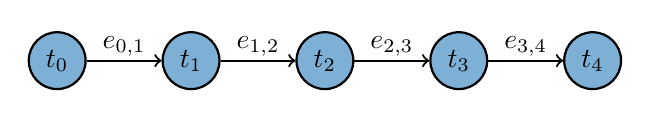
\begin{tikzpicture}[thick, node distance={17mm}, main/.style={circle,draw,fill=omni-spring-pastels-2}]
    
    \node[main] (4) {$t_0$};
    \node[main] (2) [right of=4] {$t_1$};
    \node[main] (1) [right of=2] {$t_2$};
    \node[main] (0) [right of=1] {$t_3$};
    \node[main] (3) [right of=0] {$t_4$};
    
    \draw[->] (4) -- (2) node[midway, yshift=5] {$e_{0,1}$};
    \draw[->] (2) -- (1) node[midway, yshift=5] {$e_{1,2}$};
    \draw[->] (1) -- (0) node[midway, yshift=5] {$e_{2,3}$};
    \draw[->] (0) -- (3) node[midway, yshift=5] {$e_{3,4}$};
    
\end{tikzpicture}

        }
    \end{figure}
    
    \vspace{10pt}
    \begin{columns}
        \column{.45\linewidth}
        \centering Contiguous mapping
        \begin{figure}
            \centering
            \resizebox{.4\linewidth}{!}{
                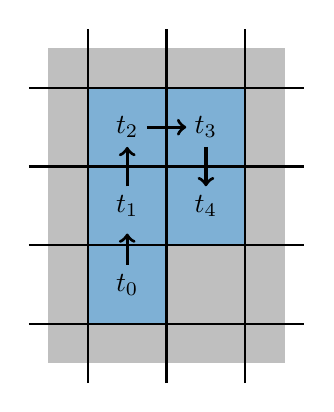
\begin{tikzpicture}[thick]
    \fill[gray!50](0.5,0.5) rectangle (3.5, 4.5); ;
    \draw[step=1 cm, color=black] (0.25, 0.25) grid (3.75, 4.75);
    
    \node[fill=omni-spring-pastels-2, minimum size=1 cm, draw=black] (1) at (1.5, 1.5) {\textbf{$t_0$}};
    \node[fill=omni-spring-pastels-2, minimum size=1 cm, draw=black] (3) at (1.5, 2.5) {\textbf{$t_1$}};
    \node[fill=omni-spring-pastels-2, minimum size=1 cm, draw=black] (2) at (1.5, 3.5) {\textbf{$t_2$}};
    \node[fill=omni-spring-pastels-2, minimum size=1 cm, draw=black] (4) at (2.5, 3.5) {\textbf{$t_3$}};
    \node[fill=omni-spring-pastels-2, minimum size=1 cm, draw=black] (5) at (2.5, 2.5) {\textbf{$t_4$}};
    

    \coordinate (2t1) at (1.5, 2.75) ;
    \coordinate (1f2) at (1.5, 3.25) ;
    \draw[->, very thick] (2t1) -- (1f2);
    
    \coordinate (4t2) at (1.5, 1.75) ;
    \coordinate (2f4) at (1.5, 2.15) ;
    \draw[->, very thick] (4t2) -- (2f4);

    \coordinate (1t0) at (1.75, 3.5) ;
    \coordinate (0f1) at (2.25, 3.5) ;
    \draw[->, very thick] (1t0) -- (0f1);
    
    
    \coordinate (0t3) at (2.5, 3.25) ;
    \coordinate (3f0) at (2.5, 2.75) ;
    \draw[->, very thick] (0t3) -- (3f0);

\end{tikzpicture}

            }
        \end{figure}

        \column{.45\linewidth}
        \centering Non-Contiguous mapping
        \begin{figure}
            \centering
            \resizebox{.5\linewidth}{!}{
                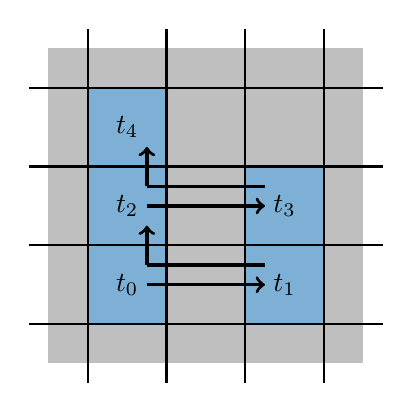
\begin{tikzpicture}[thick]
    \fill[gray!50](0.5,0.5) rectangle (4.5, 4.5); ;
    \draw[step=1 cm, color=black] (0.25, 0.25) grid (4.75, 4.75);
    
    \node[fill=omni-spring-pastels-2, minimum size=1 cm, draw=black] (1) at (1.5, 1.5) {\textbf{$t_0$}};
    \node[fill=omni-spring-pastels-2, minimum size=1 cm, draw=black] (3) at (3.5, 1.5) {\textbf{$t_1$}};
    \node[fill=omni-spring-pastels-2, minimum size=1 cm, draw=black] (2) at (1.5, 2.5) {\textbf{$t_2$}};
    \node[fill=omni-spring-pastels-2, minimum size=1 cm, draw=black] (4) at (3.5, 2.5) {\textbf{$t_3$}};
    \node[fill=omni-spring-pastels-2, minimum size=1 cm, draw=black] (5) at (1.5, 3.5) {\textbf{$t_4$}};

    \coordinate (4t2) at (1.75, 1.5) ;
    \coordinate (2f4) at (3.25, 1.5) ;
    \draw[->, very thick] (4t2) -- (2f4);

    \coordinate (2t4t2) at (3.25, 1.75) ;
    \coordinate (4f2)   at (1.75, 1.75) ;
    \coordinate (1f4f2) at (1.75, 2.25) ;
    \draw[-, very thick] (2t4t2) -- (4f2);
    \draw[->, very thick] (4f2) -- (1f4f2);

    \coordinate (1t0) at (1.75, 2.5) ;
    \coordinate (0f1) at (3.25, 2.5) ;
    \draw[->, very thick] (1t0) -- (0f1);
    
    \coordinate (0t1t3) at (3.25, 2.75) ;
    \coordinate (1f0)   at (1.75, 2.75) ;
    \coordinate (3f1f0) at (1.75, 3.25) ;
    \draw[-, very thick] (0t1t3) -- (1f0);
    \draw[->, very thick] (1f0) -- (3f1f0);

\end{tikzpicture}

            }
        \end{figure}
    \end{columns}
\end{frame}

\begin{frame}{Application profile}
    \centering Communication behavior

    \begin{figure}[!ht]
        \centering
        \resizebox{.75\linewidth}{!}{
            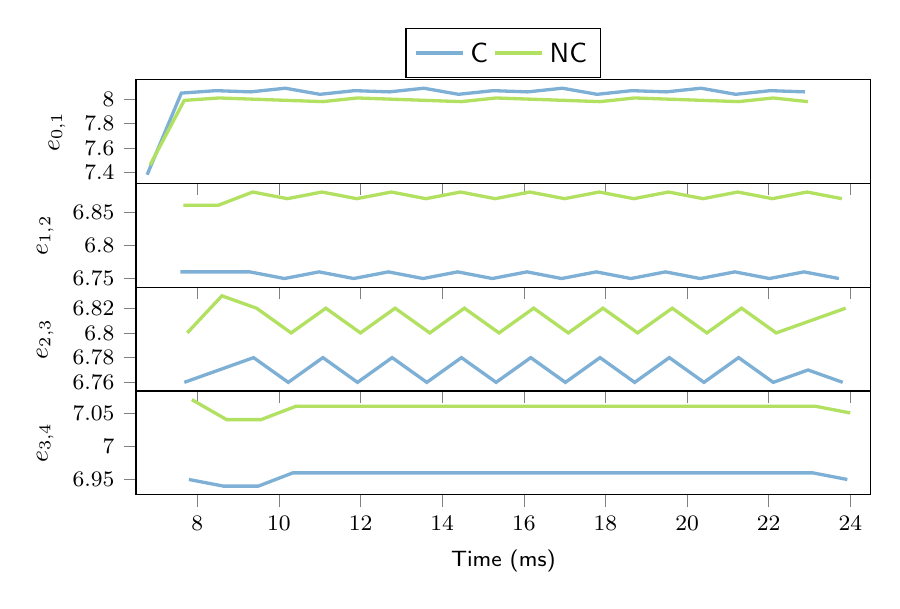
\begin{tikzpicture}
    \begin{groupplot}[
        group style={
            group name=my plots,
            group size=1 by 4,
            xlabels at=edge bottom,
            xticklabels at=edge bottom,
            vertical sep=0pt
        },
        small,
        width=.9\linewidth,
        height=2.9cm,
        xlabel={\footnotesize Time (ms)},
        xmin=6.5, xmax=24.5,
        % grid=major,
        tickpos=left,
        ytick align=outside,
        xtick align=outside,
    ]
        \nextgroupplot [
            ylabel={$e_{0,1}$ \scriptsize}, 
            legend style={
                at={(0.5,1.5)}, 
                anchor=north,
                legend columns=3
            },
        ]
        \addplot+ [mark=none, omni-spring-pastels-2, very thick] coordinates{
            (6.7724, 7.38)
            (7.61006, 8.05)
            (8.45949, 8.07)
            (9.30819, 8.06)
            (10.15691, 8.09)
            (11.00561, 8.04)
            (11.85433, 8.07)
            (12.70303, 8.06)
            (13.55175, 8.09)
            (14.40045, 8.04)
            (15.24917, 8.07)
            (16.09787, 8.06)
            (16.94659, 8.09)
            (17.79529, 8.04)
            (18.64401, 8.07)
            (19.49271, 8.06)
            (20.34143, 8.09)
            (21.19013, 8.04)
            (22.03885, 8.07)
            (22.88755, 8.06)        
        };

        \addplot+ [mark=none, omni-spring-pastels-3, very thick] coordinates{
            (6.84402, 7.46)
            (7.68168, 7.99)
            (8.53111, 8.01)
            (9.37981, 8.0)
            (10.22853, 7.99)
            (11.07723, 7.98)
            (11.92595, 8.01)
            (12.77465, 8.0)
            (13.62337, 7.99)
            (14.47207, 7.98)
            (15.32079, 8.01)
            (16.16949, 8.0)
            (17.01821, 7.99)
            (17.86691, 7.98)
            (18.71563, 8.01)
            (19.56433, 8.0)
            (20.41305, 7.99)
            (21.26175, 7.98)
            (22.11047, 8.01)
            (22.95917, 7.98)
        };

        \legend{\strut C, \strut NC}
        
        \nextgroupplot [ylabel={$e_{1,2}$ \scriptsize}]
        \addplot+ [mark=none, omni-spring-pastels-2, very thick] coordinates{
            (7.58932, 6.76)
            (8.43875, 6.76)
            (9.28745, 6.76)
            (10.13616, 6.75)
            (10.98487, 6.76)
            (11.83358, 6.75)
            (12.68229, 6.76)
            (13.531, 6.75)
            (14.37971, 6.76)
            (15.22842, 6.75)
            (16.07713, 6.76)
            (16.92584, 6.75)
            (17.77455, 6.76)
            (18.62326, 6.75)
            (19.47197, 6.76)
            (20.32068, 6.75)
            (21.16939, 6.76)
            (22.0181, 6.75)
            (22.86681, 6.76)
            (23.72004, 6.75)
        };

        \addplot+ [mark=none, omni-spring-pastels-3, very thick] coordinates{
            (7.66104, 6.86)
            (8.51047, 6.86)
            (9.35919, 6.88)
            (10.2079, 6.87)
            (11.05661, 6.88)
            (11.90532, 6.87)
            (12.75403, 6.88)
            (13.60274, 6.87)
            (14.45145, 6.88)
            (15.30016, 6.87)
            (16.14887, 6.88)
            (16.99758, 6.87)
            (17.84629, 6.88)
            (18.695, 6.87)
            (19.54371, 6.88)
            (20.39242, 6.87)
            (21.24113, 6.88)
            (22.08984, 6.87)
            (22.93855, 6.88)
            (23.79178, 6.87)
        };
        
        \nextgroupplot [ylabel={$e_{2,3}$}] %[ylabel={\footnotesize Latency (us)}, ylabel shift = -30 pt, every axis y label/.append style={at=(ticklabel cs:1.0)}]
        \addplot+ [mark=none, omni-spring-pastels-2, very thick] coordinates{
            (7.68254, 6.76)
            (8.5323, 6.77)
            (9.38028, 6.78)
            (10.22899, 6.76)
            (11.0777, 6.78)
            (11.92641, 6.76)
            (12.77512, 6.78)
            (13.62383, 6.76)
            (14.47254, 6.78)
            (15.32125, 6.76)
            (16.16996, 6.78)
            (17.01867, 6.76)
            (17.86738, 6.78)
            (18.71609, 6.76)
            (19.5648, 6.78)
            (20.41351, 6.76)
            (21.26222, 6.78)
            (22.11093, 6.76)
            (22.96415, 6.77)
            (23.81287, 6.76)
        };

        \addplot+ [mark=none, omni-spring-pastels-3, very thick] coordinates{
            (7.7543, 6.8)
            (8.60408, 6.83)
            (9.45206, 6.82)
            (10.30077, 6.8)
            (11.14948, 6.82)
            (11.99819, 6.8)
            (12.8469, 6.82)
            (13.69561, 6.8)
            (14.54432, 6.82)
            (15.39303, 6.8)
            (16.24174, 6.82)
            (17.09045, 6.8)
            (17.93916, 6.82)
            (18.78787, 6.8)
            (19.63658, 6.82)
            (20.48529, 6.8)
            (21.334, 6.82)
            (22.18271, 6.8)
            (23.03593, 6.81)
            (23.88467, 6.82)
        };

        \nextgroupplot [ylabel={$e_{3,4}$ \scriptsize}]
        \addplot+ [mark=none, omni-spring-pastels-2, very thick] coordinates{
            (7.79647, 6.95)
            (8.64654, 6.94)
            (9.49379, 6.94)
            (10.34254, 6.96)
            (11.19123, 6.96)
            (12.03996, 6.96)
            (12.88865, 6.96)
            (13.73738, 6.96)
            (14.58607, 6.96)
            (15.4348, 6.96)
            (16.28349, 6.96)
            (17.13222, 6.96)
            (17.98091, 6.96)
            (18.82964, 6.96)
            (19.67833, 6.96)
            (20.52706, 6.96)
            (21.37575, 6.96)
            (22.22448, 6.96)
            (23.07768, 6.96)
            (23.92641, 6.95)
        };

        \addplot+ [mark=none, omni-spring-pastels-3, very thick] coordinates{
            (7.86835, 7.07)
            (8.71842, 7.04)
            (9.56567, 7.04)
            (10.41442, 7.06)
            (11.26311, 7.06)
            (12.11184, 7.06)
            (12.96053, 7.06)
            (13.80926, 7.06)
            (14.65795, 7.06)
            (15.50668, 7.06)
            (16.35537, 7.06)
            (17.2041, 7.06)
            (18.05279, 7.06)
            (18.90152, 7.06)
            (19.75021, 7.06)
            (20.59894, 7.06)
            (21.44763, 7.06)
            (22.29636, 7.06)
            (23.14956, 7.06)
            (23.99831, 7.05)
        };
        
    \end{groupplot}    
\end{tikzpicture}

        }
    \end{figure}
\end{frame}

\begin{frame}{Application profile}
    \centering Mapping with Disturbing traffic
    \begin{figure}
        \centering
        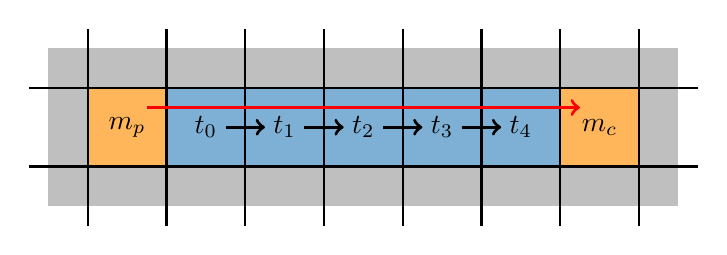
\begin{tikzpicture}[thick]

    \fill[gray!50](0.5,0.5) rectangle (8.5, 2.5); ;
    \draw[step=1 cm, color=black] (0.25, 0.25) grid (8.75, 2.75);
    
    \node[fill=omni-spring-pastels-2, minimum size=1 cm, draw=black] (1) at (2.5, 1.5) {\textbf{$t_0$}};
    \node[fill=omni-spring-pastels-2, minimum size=1 cm, draw=black] (3) at (3.5, 1.5) {\textbf{$t_1$}};
    \node[fill=omni-spring-pastels-2, minimum size=1 cm, draw=black] (2) at (4.5, 1.5) {\textbf{$t_2$}};
    \node[fill=omni-spring-pastels-2, minimum size=1 cm, draw=black] (4) at (5.5, 1.5) {\textbf{$t_3$}};
    \node[fill=omni-spring-pastels-2, minimum size=1 cm, draw=black] (5) at (6.5, 1.5) {\textbf{$t_4$}};
    

    \coordinate (4t2) at (2.75, 1.5) ;
    \coordinate (2f4) at (3.25, 1.5) ;
    \draw[->, very thick] (4t2) -- (2f4);
    
    \coordinate (2t1) at (3.75, 1.5) ;
    \coordinate (1f2) at (4.25, 1.5) ;
    \draw[->, very thick] (2t1) -- (1f2);

    \coordinate (1t0) at (4.75, 1.5) ;
    \coordinate (0f1) at (5.25, 1.5) ;
    \draw[->, very thick] (1t0) -- (0f1);
    
    
    \coordinate (0t3) at (5.75, 1.5) ;
    \coordinate (3f0) at (6.25, 1.5) ;
    \draw[->, very thick] (0t3) -- (3f0);

    \node[fill=omni-spring-pastels-5, minimum size=1 cm, draw=black] (6) at (1.5, 1.5) {\textbf{$m_p$}};
    \node[fill=omni-spring-pastels-5, minimum size=1 cm, draw=black] (7) at (7.5, 1.5) {\textbf{$m_c$}};

    \coordinate (ptc) at (1.75, 1.75) ;
    \coordinate (cfp) at (7.25, 1.75) ;
    \draw[red, ->, very thick] (ptc) -- (cfp);
\end{tikzpicture}

    \end{figure}

    \begin{itemize}
        \item $m_p$ sends messages to $m_c$
        \item Random intervals (100-500 $\mu s$)
        \item 96 flits per message        
    \end{itemize}
\end{frame}

\begin{frame}{Application profiling}
    \centering Communication behavior

    \begin{figure}[!ht]
        \centering
        \resizebox{0.75\linewidth}{!}{
            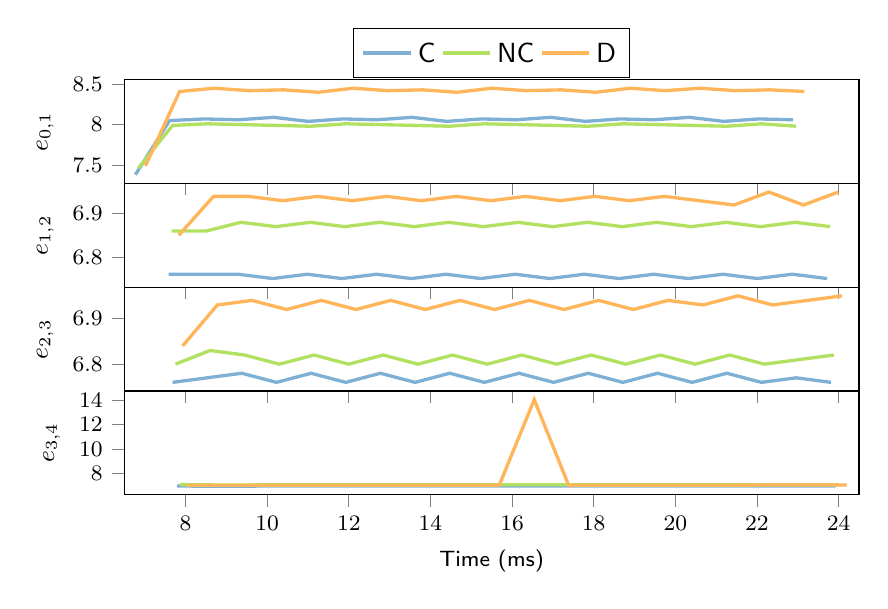
\begin{tikzpicture}
    \begin{groupplot}[
        group style={
            group name=my plots,
            group size=1 by 4,
            xlabels at=edge bottom,
            xticklabels at=edge bottom,
            vertical sep=0pt
        },
        small,
        width=.9\linewidth,
        height=2.9cm,
        xlabel={\footnotesize Time (ms)},
        xmin=6.5, xmax=24.5,
        % grid=major,
        tickpos=left,
        ytick align=outside,
        xtick align=outside,
    ]
        \nextgroupplot [
            ylabel={$e_{0,1}$ \scriptsize}, 
            legend style={
                at={(0.5,1.5)}, 
                anchor=north,
                legend columns=3
            },
        ]
        \addplot+ [mark=none, omni-spring-pastels-2, very thick] coordinates{
            (6.7724, 7.38)
            (7.61006, 8.05)
            (8.45949, 8.07)
            (9.30819, 8.06)
            (10.15691, 8.09)
            (11.00561, 8.04)
            (11.85433, 8.07)
            (12.70303, 8.06)
            (13.55175, 8.09)
            (14.40045, 8.04)
            (15.24917, 8.07)
            (16.09787, 8.06)
            (16.94659, 8.09)
            (17.79529, 8.04)
            (18.64401, 8.07)
            (19.49271, 8.06)
            (20.34143, 8.09)
            (21.19013, 8.04)
            (22.03885, 8.07)
            (22.88755, 8.06)        
        };

        \addplot+ [mark=none, omni-spring-pastels-3, very thick] coordinates{
            (6.84402, 7.46)
            (7.68168, 7.99)
            (8.53111, 8.01)
            (9.37981, 8.0)
            (10.22853, 7.99)
            (11.07723, 7.98)
            (11.92595, 8.01)
            (12.77465, 8.0)
            (13.62337, 7.99)
            (14.47207, 7.98)
            (15.32079, 8.01)
            (16.16949, 8.0)
            (17.01821, 7.99)
            (17.86691, 7.98)
            (18.71563, 8.01)
            (19.56433, 8.0)
            (20.41305, 7.99)
            (21.26175, 7.98)
            (22.11047, 8.01)
            (22.95917, 7.98)
        };

        \addplot+ [mark=none, omni-spring-pastels-5, very thick] coordinates{
            (7.01808, 7.49)
            (7.85639, 8.41)
            (8.707, 8.45)
            (9.55634, 8.42)
            (10.4057, 8.43)
            (11.25504, 8.4)
            (12.1044, 8.45)
            (12.95374, 8.42)
            (13.8031, 8.43)
            (14.65244, 8.4)
            (15.5018, 8.45)
            (16.35114, 8.42)
            (17.2005, 8.43)
            (18.04984, 8.4)
            (18.8992, 8.45)
            (19.74854, 8.42)
            (20.60694, 8.45)
            (21.46152, 8.42)
            (22.31088, 8.43)
            (23.16022, 8.41)
        };

        \legend{\strut C, \strut NC, \strut D}
        
        \nextgroupplot [ylabel={$e_{1,2}$ \scriptsize}]
        \addplot+ [mark=none, omni-spring-pastels-2, very thick] coordinates{
            (7.58932, 6.76)
            (8.43875, 6.76)
            (9.28745, 6.76)
            (10.13616, 6.75)
            (10.98487, 6.76)
            (11.83358, 6.75)
            (12.68229, 6.76)
            (13.531, 6.75)
            (14.37971, 6.76)
            (15.22842, 6.75)
            (16.07713, 6.76)
            (16.92584, 6.75)
            (17.77455, 6.76)
            (18.62326, 6.75)
            (19.47197, 6.76)
            (20.32068, 6.75)
            (21.16939, 6.76)
            (22.0181, 6.75)
            (22.86681, 6.76)
            (23.72004, 6.75)
        };

        \addplot+ [mark=none, omni-spring-pastels-3, very thick] coordinates{
            (7.66104, 6.86)
            (8.51047, 6.86)
            (9.35919, 6.88)
            (10.2079, 6.87)
            (11.05661, 6.88)
            (11.90532, 6.87)
            (12.75403, 6.88)
            (13.60274, 6.87)
            (14.45145, 6.88)
            (15.30016, 6.87)
            (16.14887, 6.88)
            (16.99758, 6.87)
            (17.84629, 6.88)
            (18.695, 6.87)
            (19.54371, 6.88)
            (20.39242, 6.87)
            (21.24113, 6.88)
            (22.08984, 6.87)
            (22.93855, 6.88)
            (23.79178, 6.87)
        };

        \addplot+ [mark=none, omni-spring-pastels-5, very thick] coordinates{
            (7.83542, 6.85)
            (8.68612, 6.94)
            (9.53546, 6.94)
            (10.38481, 6.93)
            (11.23416, 6.94)
            (12.08351, 6.93)
            (12.93286, 6.94)
            (13.78221, 6.93)
            (14.63156, 6.94)
            (15.48091, 6.93)
            (16.33026, 6.94)
            (17.17961, 6.93)
            (18.02896, 6.94)
            (18.87831, 6.93)
            (19.72766, 6.94)
            (20.58605, 6.93)
            (21.44062, 6.92)
            (22.29001, 6.95)
            (23.13932, 6.92)
            (23.99323, 6.95)
        };
        
        \nextgroupplot [ylabel={$e_{2,3}$}] %[ylabel={\footnotesize Latency (us)}, ylabel shift = -30 pt, every axis y label/.append style={at=(ticklabel cs:1.0)}]
        \addplot+ [mark=none, omni-spring-pastels-2, very thick] coordinates{
            (7.68254, 6.76)
            (8.5323, 6.77)
            (9.38028, 6.78)
            (10.22899, 6.76)
            (11.0777, 6.78)
            (11.92641, 6.76)
            (12.77512, 6.78)
            (13.62383, 6.76)
            (14.47254, 6.78)
            (15.32125, 6.76)
            (16.16996, 6.78)
            (17.01867, 6.76)
            (17.86738, 6.78)
            (18.71609, 6.76)
            (19.5648, 6.78)
            (20.41351, 6.76)
            (21.26222, 6.78)
            (22.11093, 6.76)
            (22.96415, 6.77)
            (23.81287, 6.76)
        };

        \addplot+ [mark=none, omni-spring-pastels-3, very thick] coordinates{
            (7.7543, 6.8)
            (8.60408, 6.83)
            (9.45206, 6.82)
            (10.30077, 6.8)
            (11.14948, 6.82)
            (11.99819, 6.8)
            (12.8469, 6.82)
            (13.69561, 6.8)
            (14.54432, 6.82)
            (15.39303, 6.8)
            (16.24174, 6.82)
            (17.09045, 6.8)
            (17.93916, 6.82)
            (18.78787, 6.8)
            (19.63658, 6.82)
            (20.48529, 6.8)
            (21.334, 6.82)
            (22.18271, 6.8)
            (23.03593, 6.81)
            (23.88467, 6.82)
        };

        \addplot+ [mark=none, omni-spring-pastels-5, very thick] coordinates{
            (7.92905, 6.84)
            (8.78027, 6.93)
            (9.62835, 6.94)
            (10.4777, 6.92)
            (11.32705, 6.94)
            (12.1764, 6.92)
            (13.02575, 6.94)
            (13.8751, 6.92)
            (14.72445, 6.94)
            (15.5738, 6.92)
            (16.42315, 6.94)
            (17.2725, 6.92)
            (18.12185, 6.94)
            (18.9712, 6.92)
            (19.82055, 6.94)
            (20.67895, 6.93)
            (21.53352, 6.95)
            (22.38291, 6.93)
            (23.23673, 6.94)
            (24.08615, 6.95)
        };

        \nextgroupplot [ylabel={$e_{3,4}$ \scriptsize}]
        \addplot+ [mark=none, omni-spring-pastels-2, very thick] coordinates{
            (7.79647, 6.95)
            (8.64654, 6.94)
            (9.49379, 6.94)
            (10.34254, 6.96)
            (11.19123, 6.96)
            (12.03996, 6.96)
            (12.88865, 6.96)
            (13.73738, 6.96)
            (14.58607, 6.96)
            (15.4348, 6.96)
            (16.28349, 6.96)
            (17.13222, 6.96)
            (17.98091, 6.96)
            (18.82964, 6.96)
            (19.67833, 6.96)
            (20.52706, 6.96)
            (21.37575, 6.96)
            (22.22448, 6.96)
            (23.07768, 6.96)
            (23.92641, 6.95)
        };

        \addplot+ [mark=none, omni-spring-pastels-3, very thick] coordinates{
            (7.86835, 7.07)
            (8.71842, 7.04)
            (9.56567, 7.04)
            (10.41442, 7.06)
            (11.26311, 7.06)
            (12.11184, 7.06)
            (12.96053, 7.06)
            (13.80926, 7.06)
            (14.65795, 7.06)
            (15.50668, 7.06)
            (16.35537, 7.06)
            (17.2041, 7.06)
            (18.05279, 7.06)
            (18.90152, 7.06)
            (19.75021, 7.06)
            (20.59894, 7.06)
            (21.44763, 7.06)
            (22.29636, 7.06)
            (23.14956, 7.06)
            (23.99831, 7.05)
        };

        \addplot+ [mark=none, omni-spring-pastels-5, very thick] coordinates{
            (8.04348, 7.01)
            (8.89503, 7.02)
            (9.74184, 7.02)
            (10.59121, 7.02)
            (11.44054, 7.02)
            (12.28991, 7.02)
            (13.13924, 7.02)
            (13.98861, 7.02)
            (14.83794, 7.02)
            (15.68731, 7.02)
            (16.54366, 14.04)
            (17.38601, 7.02)
            (18.23534, 7.02)
            (19.08471, 7.02)
            (19.93404, 7.02)
            (20.79246, 7.02)
            (21.64701, 7.02)
            (22.49644, 7.04)
            (23.35024, 7.04)
            (24.19967, 7.03)
        };
        
    \end{groupplot}    
\end{tikzpicture}

        }
    \end{figure}
\end{frame}

\begin{frame}{Application profile}
    \begin{itemize}
        \item An application has a communication behavior for each of its edges
        \item The behavior does not change with the number of hops between edges
    \end{itemize}

    \vspace{0.5cm}
    \textit{This behavior cannot be captured by models that only monitor latency, which was adopted in early work}

    \begin{alertblock}{Challenge}
        Develop an application profile capable of monitoring the latency of each edge in the NoC to detect potential malicious interferences using ML
    \end{alertblock}
\end{frame}
\section{A Framework for Pre-Runtime RT Analysis}

\begin{frame}{Baseline Platform - Hardware}
	\begin{itemize}
		\item xablau
	\end{itemize}
\end{frame}
\section{Proof-of-Concept and Results}

\begin{frame}{Experimentation Setup}
  
  \begin{itemize}
  	\item We experiment on the SAE (synthetic) application whose minimum frequency to meet its RT requirements is known ($500$MHz).
  	\item We map SAE to a 2x2 instance of our manycore
	\item We perform clustering using the \textit{max-proc} criterion and $n = 4$.
	\item The nominal frequency of our platform is $2.5$GHz, which is also given as input to our framework. 
	\item By the last iteration, our framework found $500.4$MHz as the minimum frequency to meet the RT constraints on the platform. Since we cannot display the results for all iterations, we couple to show the last step and demonstrate how the found frequency meets the requirement of the application (the last frequency).
  \end{itemize}
  
\end{frame}


\begin{frame}
	
	\begin{itemize}
		\item The CPA method estimated the end-to-end iteration execution time of SAE based on the application graph and the WCET of the kernel operations. 
		
		\item Our scheduler has a WCET of $110$ kcycles, and our network driver has a WCET of $20$ kcycles. Tasks are scheduled once per iteration due to our PBRR implementation. The total iteration execution time, as pointed out by the CPA method, is $8.464.895$ cycles. 
		
		\item The actual RTL execution is $6.799.200$ cycles ($80\%$). The CPA method overestimates $\simeq 26\%$ of the actual CPU usage. However, the overestimation is \textit{acceptable} ($<30\%$) as the actual CPU usage stays below  $70\%$; a CPU usage over $70\%$ is often considered questionable~\cite{Ovaska:2011}.
		
	\end{itemize}
	

\end{frame}

\begin{frame}{}
    
    \vspace{-0.8em}
    \begin{table}[!ht]
    	\caption{Comparison of Execution time (CPU).}
    	\label{tab:results}
    	\centering
    	\resizebox{1\textwidth}{!}{%
    		\begin{tabular}{lrrrrr}
    			\toprule
    			\textbf{Cluster} & \textbf{Execution$^1$} & \textbf{Estimation$^2$} & \textbf{Difference} & \textbf{Diff. (\%)$^3$} & \textbf{Usage$^4$}\\
    			\cmidrule(lr){1-1}
    			\cmidrule(lr){2-2}
    			\cmidrule(lr){3-3}
    			\cmidrule(lr){4-4}
    			\cmidrule(lr){5-5}
    			\cmidrule(lr){6-6}
    			
    			\rowcolor{\rowcolordark} 
    			ABDF & $1,439,000$ & $1,819,300$ & $+380,300$ & $+26.428\%$ & $72.722\%$\\
    			
    			C & $801,300$ & $963,300$ & $+162.000$ & $+20.217\%$  & $38.532\%$\\
    			
    			\rowcolor{\rowcolordark} 
    			EHI & $2,174,500$ & $2,667,895$ & $+493,395$ &  $+22.690\%$  & $71.616\%$\\
    			
    			GJ & $2,384,400$ & $3,014,400$ & $+630.000$ & $+26.421\%$ & $86.980\%$\\     
    			
    			\bottomrule
    			\multicolumn{6}{p{9.5cm}}{\footnotesize{$^1$Execution time (RTL, cycles); $^2$CPA estimation; $^3$Execution time is $100\%$; $^4$DES.}}
    		\end{tabular}
    		
    	} % end of resize box
    \end{table}
    \vspace{-0.8em}
\end{frame}


\begin{frame}
	
	\begin{itemize}
		
		\item The framework captured the time that tasks finished during the DES simulation. As tasks implement the PREM and LET models, we assume that packets are injected at the same time they leave the CPU.
		
		\item Table~\ref{tab:flows} shows the characterization of flows, where $ph$ is the phase time (the period of scheduling interrupts), $pv$ is the \textit{phase} of the task, and $\psi = (ph \times pv)$. 
		
		\item A phase corresponds to the alignment of application execution to the scheduler tick. For instance, the SAE application cannot finish before the $4^{th}$ phase due to the critical path traverses 4 tasks in the application graph. This is a necessary step, as the DES simulation does not account for task dependency. Deadlines match the end of the phase of the receiving task.%GRAMMARLY-OK
				
	\end{itemize}
	
\end{frame}



\begin{frame}
	
	
	\vspace{-10 pt}
	\begin{table}[!ht]
		\caption{Characterization of flows for the SAE application.}
		\label{tab:flows}
		\centering
		\resizebox{0.8\textwidth}{!}{%
			\begin{tabular}{lrccrr}
				\toprule
				\textbf{Flow} & \textbf{MRT$^1$} & \textbf{S} & \textbf{D} & \textbf{Volume} & \textbf{Deadline}\\
				\cmidrule(lr){1-1}
				\cmidrule(lr){2-2}
				\cmidrule(lr){3-3}
				\cmidrule(lr){4-4}
				\cmidrule(lr){5-5}
				\cmidrule(lr){6-6}
				
				\rowcolor{\rowcolordark} $F_1$ & $285300 + \psi$ & A & C & $12300$ & $110000 +  \psi$\\
				$F_2$ & $1819300 + \psi$ & F & G & $67800$ & $110000 + \psi$\\
				\rowcolor{\rowcolordark} $F_3$ & $963300  + \psi$ & C & E & $12000$ & $110000 + \psi$\\
				$F_4$ & $1280700 + \psi$ & I & J & $56700$ & $1208800  + \psi$\\
				\rowcolor{\rowcolordark} $F_5$ & $1733700 + \psi$ & H & J & $89000$ & $1208800 + \psi$\\
				
				\bottomrule
				\multicolumn{6}{p{7cm}}{\footnotesize{(S) source task, (D) destination task, $^1$Minimum release time.}}
			\end{tabular}
			
		} % end of resize box
		\vspace{-8 pt}
	\end{table}	
	
\end{frame}



\begin{frame}
	\begin{itemize}
		\item In Figure~\ref{fig:phases}, we present the RTL simulation of our manycore running the SAE application at the minimum frequency of $500.4$MHz, obtained from our framework. The goal is to demonstrate that the application meets its RT requirements. 
		
		\item The hyperperiod of SAE is $20$ms, corresponding to 4 phases of $5$ms each, meeting the expected iteration time and iterations per second requirements. SAE receives stimuli from outside the system once per $5$ms, triggering $4$ instances of the application per $20ms$ (Task \textsc{a}). SAE returns results to outside the system via Task \textsc{j}. 
		
		\item The $3^{\text{rd}}$ instance of the application (pink) has additional $1.457$ms in its iteration time, related to the scheduling of Task \textsc{i}; the task executes two iterations at once due to two packets received in the phase time, delaying Task \textsc{j}. Nevertheless, Task \textsc{j} meets its deadlines for all instances of SAE, for an iteration time of $16,820$ms for the $1^{\text{st}}$, $2^{\text{nd}}$ and $3^{\text{th}}$ instances, and $18.277$ms for the $3^{\text{rd}}$ instance.
	\end{itemize}
\end{frame}


\begin{frame}
	\begin{figure}[!ht]
		\centerline{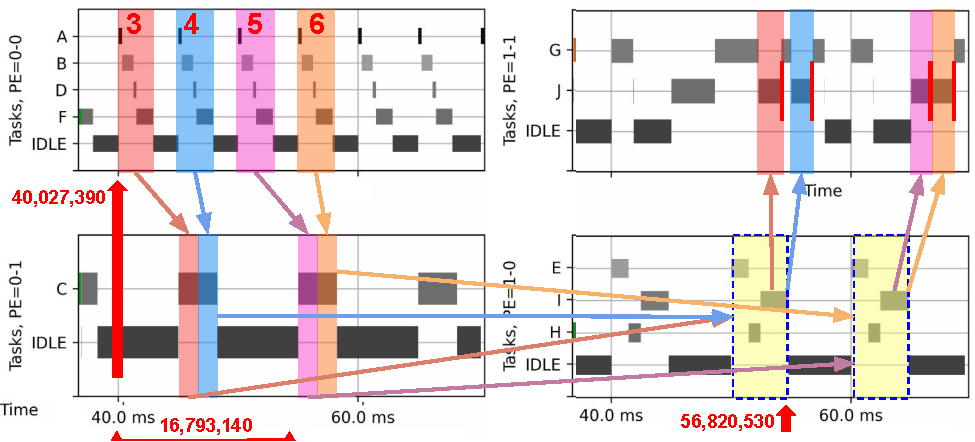
\includegraphics[width=0.8\columnwidth]{fig/results.pdf}}
		\caption{Interaction of tasks of the SAE application during RTL simulation. Rectangles with the same color represent tasks in the same iteration (instances). Arrows indicate the direction of the communication. The yellow rectangle represents a phase overlapping.}
		\vspace{-16 pt}
		\label{fig:phases}
	\end{figure}
\end{frame}
\section{Conclusions and Future Work}

\begin{frame}{Final remarks}
    \begin{columns}
        \column{.45\linewidth}
        \begin{block}{Conclusions}
            \begin{itemize}
                \item Flow for detecting anomalous traffic in NoC-based manycore systems using XGBoost
                \item Training data obtained from RTL with clock cycle accuracy
                \item Noninvasive approach -- requires only a monitoring structure
                \item High detection rate
            \end{itemize}
        \end{block}

        \column{.45\linewidth}
        \begin{block}{Future work}
            \begin{itemize}
                \item Simplify monitoring process
                \item Expand to real-time applications
                \item Enable the tuning of more hyperparameters
                \item Deploy online detection
            \end{itemize}
        \end{block}
    \end{columns}
\end{frame}

\frame[plain]{\titlepage}

\begin{frame}[allowframebreaks]{References}
    \tiny
    \bibliographystyle{alpha}
    \bibliography{bibliography}
\end{frame}

\end{document}

